\section{The Large Hadron Collider}

Located in the Lemanic basin, straddling the border between Switzerland and France, the Large Hadron Collider is the largest machine built by humans.
There are seven experiments around the circumference of the LHC: four large experiments named CMS, ALICE, LHCb, and ATLAS, as well as three small experiments named TOTEM, MoEDAL, and LHCf.
The LHC provides the unique laboratory conditions required by ATLAS to investigate the fundamental nature of the Universe.
The construction, maintenance, and operation of the LHC are part of an enormous effort carried out by thousands of dedicated scientists and engineers.
Without their ongoing endeavors, the achievements of ATLAS and the other LHC experiments would be impossible.

The LHC is impressive not just in absolute terms, but also in comparison to previous accelerators.
The three other large superconducting accelerators, the Tevatron\footnote{Decommissioned in 2011.}, HERA\footnote{Decommissioned in 2007}, and RHIC, all operate with magnetic fields of approximately 5~T.
The main dipole magnets of the LHC surpass this with fields of 8~T.
The machine is also enormous; it has a circumference of 26.7~km.
The LHC, designed to reach collision energies of 14 TeV, is also the first hadron accelerator with enough synchrotron radiation to affect the design of the cooling and vacuum systems \cite{lyndon}.

The LHC is composed of several subsystems, each of which is complex and essential in its own right.
The magnet system bends and focuses the beam to maintain its stability over multiple hours.
The accelerator system uses radio-frequency chambers to accelerate the beams.
Various control systems monitor, collimate, and adjust the kinematics of the beam.
Finally, either in the event of a problem or once the beam has lost sufficient intensity, the beam is carefully disposed in the by the abort system.
This section describes how these systems collectively provide colliding beams inside the ATLAS experiment.

The LHC is a machine under continuous development; the only place to study improvements for the LHC is at the LHC itself.
As a result, the history of the LHC development is also the history of the experimental environment of the ATLAS detector.
This story begins with the tunnel and infrastructure that houses the LHC.

\subsection{Civil Engineering}

\begin{figure}[htb]
\captionsetup[subfigure]{position=b}
\centering
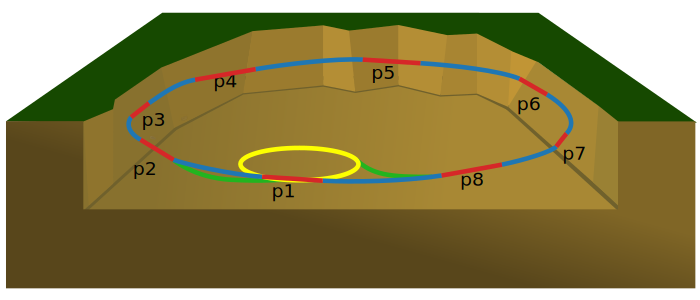
\includegraphics[width=0.9\textwidth]{figures/experiment/lhc/lhcMap.pdf}
\caption{Layout of the LHC, consisting of eight curved sections (blue) and eight straight sections (red) buried at a depth of 45-170~m. The location of SPS (yellow) and the injection lines (green) from the SPS are indicated.}
\label{figure:lhcLayout}
\end{figure}


The first step in building a collider is to construct civil infrastructure for it to inhabit.
This takes the form of a buildings that house services for the accelerator and a space for the machine itself.
For economic reasons, much of the infrastructure for the LHC is reused from the earlier LEP project.

The largest piece of infrastructure is the tunnel built to house LEP.
The Tevatron is buried less than 10~m deep in the flat expanse of the Illinois prairie.
This shallow tunnel could be constructed with a cut-and-fill approach.
RHIC is primarily built at surface level in a tunnel that was later covered with dirt.
Neither of these approaches was suitable in the context of the local geology in the region.
The land near CERN consists of a layer of moraine (loose unconsolidated rock) resting atop a layer of molasse (soft sedimentary rock).
LEP was buried in the sedimentary layer for stability, but this is too deep for excavation.
Instead, beginning in 1985, the tunnel was dug using tunnel bores and explosives.
In the Cenozoic molasse of the Lemanic basin, tunnel bores were used.
The bores were unsuitable for the fractured Mesozoic limestone beneath the Jura mountain and more costly explosives were used instead.
The resulting tunnel's internal diameter is 3.8~m, and it is buried at a depth of 45-170~m.
The tunnel slopes downward at 1.42 degrees in the direction of Lake Leman, in order to remain within the molasse layer.

The tunnel has eight curved arcs, separated by eight straight sections with length 528~m \cite{lyndon}.
Four straight sections house the ATLAS, CMS, ALICE, and LHCb experiments.
% The other four straight sections house the RF system, collimation controls, beam abort, and other utilities.
The eight straight sections, called points, are arrayed as shown in Figure \ref{figure:lhcLayout} and numbered p$i$ with $i\in\{1,...,8\}$.
The primary uses of each point is given in the following table.
\begin{center}
\begin{tabular}{c l l l}
\toprule
Location & Use \\
\midrule
    p1 & Hosts the ATLAS experiment \\
    p2 & Clockwise beam injection, and the ALICE experiment \\
    p3 & Hosts momentum collimation systems \\
    p4 & Hosts RF systems for acceleration \\
    p6 & Hosts beam abort, and beam dump \\
    p5 & Hosts the CMS and TOTEM experiments \\
    p7 & Hosts betatron collimation \\
    p8 & Counter-clockwise beam injection, and the LHCb experiment \\
\bottomrule
\end{tabular}
\end{center}
The eight curved sections host magnets with the purpose of bending the beam around the path of the machine.
The collider itself is built along the outer edge of the tunnel. In several locations, concentric outer tunnels house services for the accelerator.

After below-ground infrastructure, the next largest infrastructure for the LHC is surface buildings.
Every LEP building has been reused for the LHC, and some new infrastructure was built to accommodate the LHC.
First, a major expansion of the tunnels was undertaken to carry the beam from the SPS to the LHC injection points. Two new tunnels with an internal diameter of 3.75~m and a length of 2.5~km were dug to connect points p2 and p8 to the SPS.
While ALICE and LHCb reuse existing LEP era caverns, new caverns were built to house ATLAS and CMS.
In the cavern for CMS, the waterlogged moraine above the cavern had to be frozen with liquid nitrogen before excavation could be completed.
To avoid further flooding,\footnote{LEP flooded twice, at one time filling with 20~cm of sediment. A plan to waterproof the tunnel with a steel tube called ``the submarine'' was rejected.} existing draining tunnels were enlarged, and new tunnels were added.

In total, the construction of new infrastructure lasted five years.
\footnote{The CMS cavern construction was delayed past five years due to archaeological discoveries and the high water content of the soil. Eventually liquid nitrogen was pumped through tunnels dug through the soil to solidify it.}
Eight new surface buildings were constructed to hold offices and experimental equipment. 
Work at p1 for the three ATLAS caverns began in April of 1998 \cite{lhcDesignV2}.
Four new shafts, two over the experimental cavern and one over each service cavern, were excavated.
The ATLAS experiment cavern is built 92~m below ground. 
To house the large experiment, 300,000 tonnes of rock were removed to clear an area 53~m long, 30~m wide, and 35~m tall.
The walls and ceiling are constructed from 2~m thick concrete, and the floor is 5~m thick to support the 7,000 tonne detector.


\subsection{Accelerator Design}
The heart of the LHC is the accelerator.
The purpose of this system is to accelerate beams to their collision energy and then maintain their energy to compensate for losses over time.
% Beams are accelerated only in a short section of p4.
The circular design of the LHC means that beams repeatedly pass through the same acceleration section.
As a result, the acceleration system need only impart 3.7 kW/beam rotation.
% During the design operation, synchrotron radiation energy loss is 3.7 kW/beam: not much acceleration is lost in a revolution.
% The acceleration system needs only to make up for a small amount of lost energy per turn.

The principle of acceleration is based on radio-frequency (RF) cavities.
Independent RF systems control the acceleration of each beam circulating in opposite directions.
% Each cavity provides 32kW to increase the beam energy.
Cavities are made of copper, sputtered with niobium.\footnote{In magnetron sputtering used for this process, niobium is vaporized by particle bombardment and bound to the copper substrate of the cavity resulting in a thin - and inexpensive - 1-2 micron coating.}
This is advantageous over solid niobium for its thermal conductivity and its superconductivity to enhance the RF performance \cite{lyndon}.
The operation of the superconducting cavities requires temperatures of 4.5~k, so cavities are enclosed in cryomodules with their own helium tanks \cite{boussard}.
The resonant properties of the cavities can be adjusted during operation by mechanically distorting their shape.

Each cavity operates with a voltage of 2~MV (5.3 MV/m) and is powered by a 500~kW klystron.
The klystrons are coupled to the cavities by a waveguide of adjustable length.
Adjusting the length of the waveguide, in turn, adjusts the \emph{quality factor}\footnote{Peak energy lost per cycle, which can be used to adjust the peak voltage in the cavity.} of the cavity.
The cavity is kept at a 3~kV bias to reduce the rate of electron avalanches (multipactor effect).
During normal operation, the klystrons drive the cavities at 400~MHz and supply 200~kW.

\begin{figure}[h!]
\captionsetup[subfigure]{position=b}
\centering
    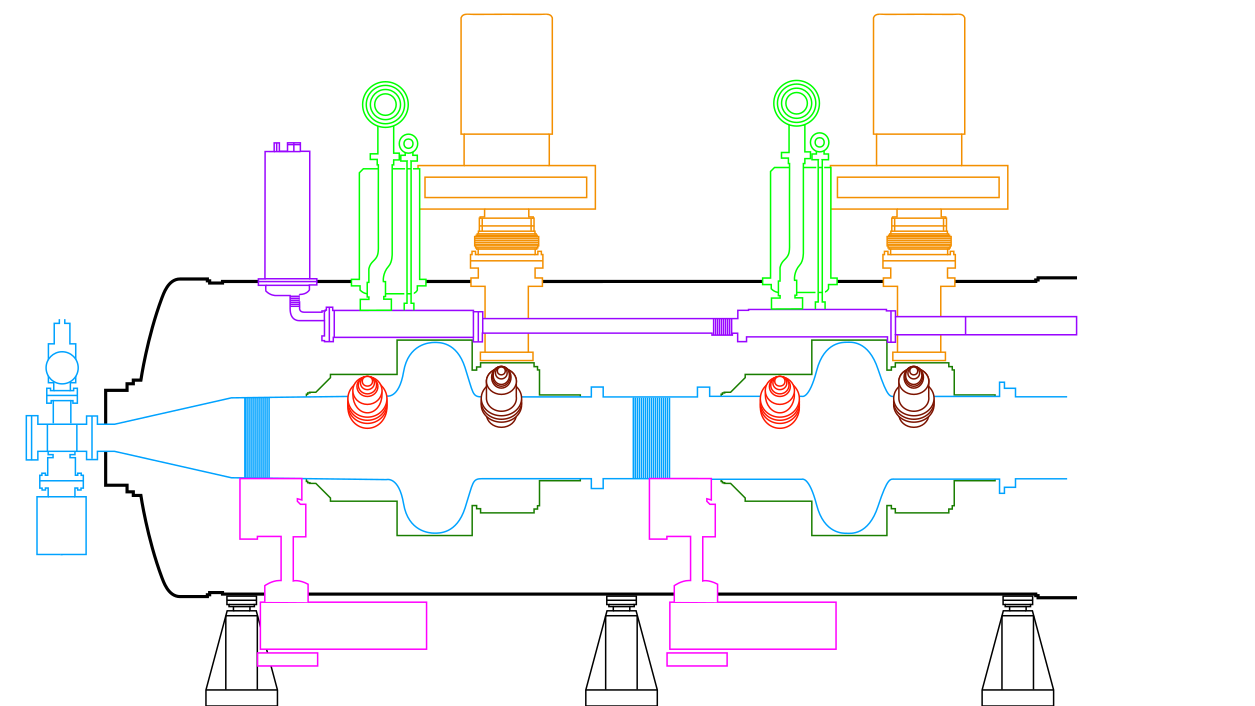
\includegraphics[width=1\textwidth]{figures/experiment/rfproto.pdf}
    % 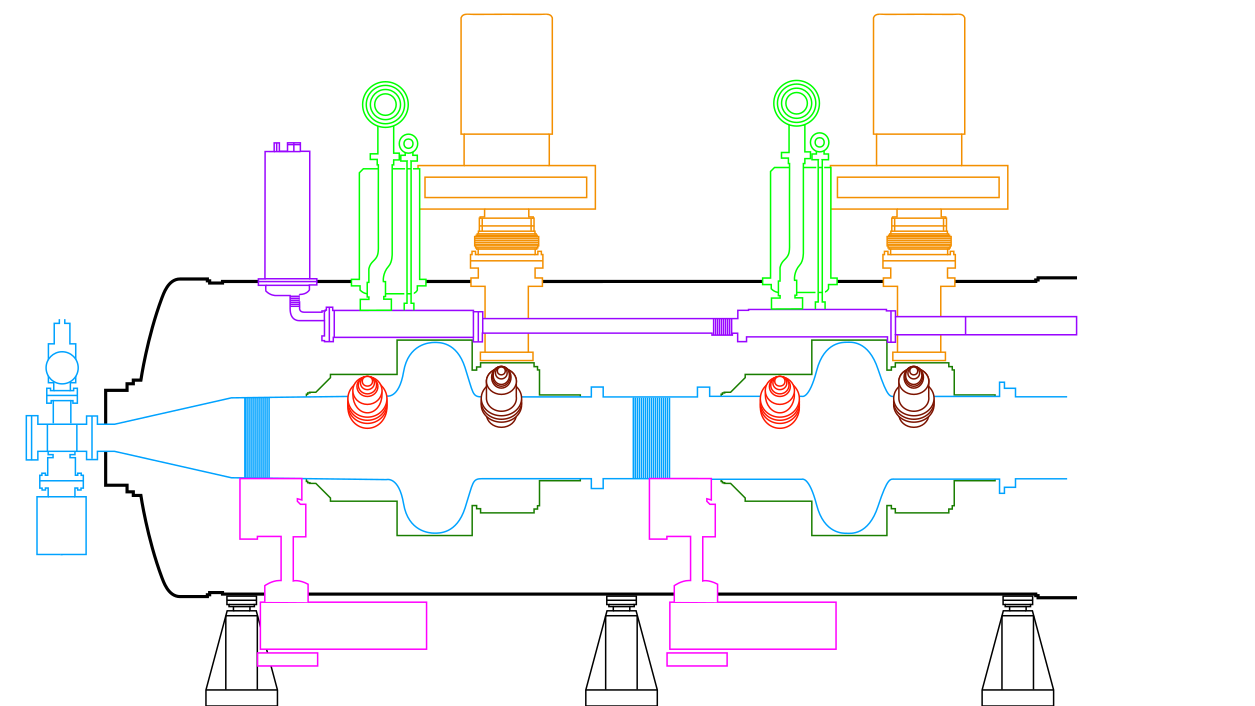
\includegraphics[width=1\textwidth]{figures/experiment/rfproto.png}
\caption{Schematic side-view of an LHC accelerating module showing two of the four cavities (blue). The cylindrical vacuum tank is shown in black. Inside, the beamline is shown in blue. The cavities are housed inside helium-filled cryomodules (dark green) fed by liquid helium baths (purple). Quench valves attached to the helium baths are shown in light green. Each super conducting cavity is driven by the variable power couplers shown in orange. Two other couplers control the higher order resonance modes in the cavity: a broadband HOM coupler (red) and a narrow band HOM coupler (brown). The resonance of each cavity is tuned by elastic deformation of the chamber by a motor system (pink).}
\label{fig:cavities}
\end{figure}

There are eight single-cell cavities per beam.
Four cavities are grouped to share a single cryostat, which maintains their superconducting temperature.
The resulting total voltage gradient is 16~MV per beam.
A schematic of the accelerator system is shown in Figure \ref{fig:cavities}.
The driving frequency is supplied through the couplings on top of the cryostat.
The cryostats are too large to sit next to each other in the tunnel, so they are staggered.

\subsection{Magnet Design}
If the accelerator is the heart of the LHC, the magnets compose its body.
Magnets serve multiple purposes in handling the beam.
A total of 1,232 dipole magnets bend the beam around the circumference of the collider.
Quadrupole magnets focus and defocus the beam as it travels. Each quadrupole simultaneously focuses in one direction and defocuses in an orthogonal direction. There are 392 quadrupoles throughout the curved arcs.
Sextupole magnets correct beam characteristics including chromaticity introduced by the quadrupoles. There are 2464 sextupole magnets in total.
Finally, other magnets such as octupole and decapole correctors fill in the remaining 7000 superconducting magnets of the LHC.
Together these magnets steer the beam into the LHC and maintain the beam's orbit during collisions.
At the end of the beam's lifetime, kicker magnets steer the beam safely into the beamdump.

\begin{figure}[h!]
\captionsetup[subfigure]{position=b}
\centering
\subcaptionbox{Coil winding \label{fig:lhcCoils}}{
    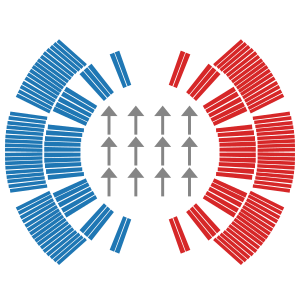
\includegraphics[width=0.4\textwidth]{figures/experiment/lhcCoils.pdf}
}
\subcaptionbox{Dipole magnet \label{fig:dipoleMagnetLhc}}{
    
\includegraphics[width=0.4\textwidth]{figures/experiment/lhcMagnet.pdf}
}
\caption{(a) Cross section of the coils made from superconductive cables wound around the beamline to produce a homogeneous dipole magnetic field. Each rectangle represents a flat Nb-Ti cable. These are grouped in a configuration that produces a smooth internal magnetic field, indicated by the arrows. The cables are separated by layers of copper. The cables are color coded: red(blue) cables carry current into(out of) the page. (b) Cross section of the main bending dipole magnets. Two beamlines (black) and coils (blue/red) are are encased by austenitic steel collars (light grey). The collar is embedded in a large iron yoke (dark grey) and submerged in a liquid helium vessel (dark blue). The arrangement is held in a cryostat. For scale, the centers of the beamlines are separated by 19~cm.
}
\label{fig:dipoleFlux}
\end{figure}

% Dipole system
The dipole magnets perform the job of bending the beam around the LHC.
Because the counter circulating beams are both positively charged, magnetic fields of opposite directions are needed to steer them.
In the dipole magnets, two sets of superconducting coils are wound from flat cables with trapezoidal cross sections.
Each cable is made from 28-36 strands of $\approx1$~mm diameter stranded niobium-titanium (Nb-Ti) alloy wires.
\footnote{Although niobium-tin (Nb$_3$Si) has many desirable advantages over Nb-Ti, it is brittle and requires many hours of heat treatment at a temperature of $\approx$970~k. Alternatively, Nb-Ti has a low heat capacity at 1.8~k, so it is susceptible to rapid heating and quenching}
The coils are arranged in inner and outer layers, as shown in Figure \ref{fig:lhcCoils}.
This configuration produces a homogeneous, purely dipole field.
The coils for each beam are positioned side-by-side, such that the field of one can augment that of the other.
These coils share a common yoke made from low carbon steel with high magnetic permeability, chosen to conduct the magnetic flux between the coils.
This is illustrated by the black arrows in Figure \ref{fig:dipoleMagnetLhc}.
The coil and yoke assembly is held in place by collar plates of austenitic (low permeability) steel.
The resulting magnetic field has an incredible strength of 8.3~T.
Each of the main dipole magnets has a length of 14.2~m (15~m, including connections between the magnets).

% Cryosystem
In order to operate at superconducting temperatures, the magnets are housed elaborate inside cryosystems that regulate their temperature.
These are challenging systems: during the LHC's Run 1, the cryosystem was responsible for 25-30\% of fault time \cite{lhcRun1}.
It is the task of the cryosystem to maintain the magnet at 1.9~K using superfluid helium. A total of 100 tons is used throughout the LHC.
Helium is used because its low viscosity allows it to permeate the coil insulation and contact directly with the superconducting wire.
Superfluid helium has a specific heat roughly 2,000 times that of the Nb-Ti; this has the important benefit of increasing the system's total specific heat.
Helium is also effective at quickly transporting heat away from the wire.
The magnets are submerged in a bath of 1~bar liquid helium. A pipe is pumped with low pressure 15~mbar liquid helium to pull heat away from the bath.
This is done to prevent vapor bubbles from developing in the bath, leading to the coil heating and subsequent quenching.
In the event of a quench, a capacitor bank is fired into series with the coil's circuit to quickly add resistivity. The current is diverted through a diode while the power is ramped down.

Magnets are grouped into ``periods'' with identical magnetic properties.
Each period is 106.9~m long and consists of six main dipoles and two 6.6~m ``short straight sections'' (SSS).
Each SSS contains quadrupole magnets that re-focus the beam after being steered by the dipoles.
Additionally, each SSS also contains sextupoles that control chromaticity and small dipoles for orbit corrections.
Some SSS also contain octupoles and trip/skew quadrupoles for fine-tuning the beam characteristics.
Perturbations in the trajectory of the beam are introduced by the magnets and are called \emph{dispersion}.
After completing one of the eight arcs, the magnet of the dispersion suppressor system cancels the horizontal dispersion introduced during the bending.

\subsection{Beam Structure and Design}
The achievement of building the LHC pales in comparison to the achievement of producing and maintaining its beams.
The LHC was designed to collide two counter-rotating beams, at precise locations, with the enormous instantaneous luminosity of $10^{34}cm^{-2}s^{-1}$.
The energy of each beam exceeds that of a large truck traveling at highway speeds.
This is more than one hundredfold the stored beam energy of any previous machine \cite{lyndon}.
The beam is an object of enormous energy and surpassing delicacy.
Numerous technical considerations must be addressed in order for the beam to be useful for the experiments.
The beams at the LHC are characterized by several parameters that describe their stability and utility.
These parameters are described in this section.

The first parameter to consider is the \emph{emittance}, $\epsilon$, defined in Equation \ref{eqn:emittance}.
It is a measure of the distribution of the particles in a beam in position-momentum phase space.
The emittance is defined as
\begin{equation}\begin{split}\label{eqn:emittance}
\epsilon \equiv \frac{6\pi}{B}\left(w^2-D^2\left(\frac{dp}{p}\right)^2\right),
\end{split}\end{equation} 
where $w$ is the RMS beam width, $D$ is the dispersion, $B\approx(w/\epsilon)$ is the beta function, and $\frac{dp}{p}$ is the relative momentum spread.
The emittance is often divided into longitudinal and transverse components.
If the emittance is too small, then intra-beam interactions destabilize the beam. 
During injection, the beam has a longitudinal emittance of 0.6-1 eV, and this is increased to 2.5 eV during acceleration for stability.
Conversely, if the transverse emittance is too large, colliding beams pass through each other without interacting.
\cite{boussard,lyndon,pdg2016}

\begin{figure}[h!]
\captionsetup[subfigure]{position=b}
\centering
\includegraphics[width=0.4\textwidth]{figures/experiment/tune.png}
\caption{Tune diagram for the LHC. The horizontal and vertical tunes are displayed. First order resonances shown in red, second order resonances shown in blue, and higher order resonances shown in black. Figure from \emph{Tune and Chromaticity Diagnostics} \cite{steinhagen}}
\label{fig:tune}
\end{figure}

Related to the transverse emittance are \emph{betatron oscillations}: harmonic motion in the transverse plane as the beam makes an orbit \cite{pdg2016}.
This is a problematic source of intra-beam scattering of protons through coulomb forces.
The frequency of betatron oscillations is higher than that of the orbit.
The number of vertical or horizontal betatron oscillations made during one orbit is called the vertical or horizontal \emph{tune}, respectively.
The horizontal and vertical tunes must be carefully picked using a tune diagram, as exemplified in Figure \ref{fig:tune}.
Resonances are illustrated as lines, and the tunes must be selected together to avoid disruptive resonances.
The beam density, $N$, as well as emittance and $\beta$ modify the tune tune $Q$:
\begin{equation}\begin{split}
    \delta Q\propto-\frac{N}{\beta\gamma^2\epsilon^*}.
\end{split}\end{equation} 
For example, when the PSB was renovated the emittance was reduced, and the energy ($\gamma$) was increased to compensate for the impact on tune.
In practice, tunes are adjusted continually by adjusting these parameters throughout beam injection, ramping up beam energy, and eventual collisions.

Related to the longitudinal emittance are \emph{synchrotron oscillations}: longitudinal oscillations along the direction of the beam.
This takes place at a much lower frequency than that of betatron oscillations: at the LHC it is less than one oscillation per orbit.
As with betatron oscillations, the synchrotron oscillation frequency must be carefully controlled to limit intra-beam scattering and maintain beam stability \cite{pdg2016}.

\emph{Chromaticity} describes the dependence of the tune on a change of momentum.
In optics, light rays of different wavelengths are focused differently by a glass focusing lens.
There is a persistent analogy between optics and beam dynamics (often called beam optics). Like light, beams are bent and focused by magnets. 
Particles with large momentum experience weaker focusing strength from focusing quadrupoles, a process called \emph{chromatic aberration}.
Chromaticity quantifies this momentum dependence.
To put it explicitly, chromaticity $Q'$ is the tune change $\Delta Q$ caused by a relative momentum change $\Delta p/p$ \cite{fuchsberger}.
\begin{equation}
    \Delta Q = Q'\frac{\Delta p}{p},
\end{equation}
where
\begin{equation}
\begin{split}
    \frac{\Delta p}{p} = \frac{\Delta f/f}{\eta}; \quad\text{and}\quad \eta = \frac{1}{\gamma_r}-\alpha_c. \\
\end{split}
\end{equation}
Here, $\Delta f$ is change in RF frequency, and $f$ is the nominal frequency \footnote{400,788,860 Hz at the LHC.} 
$\gamma_r$ is relativistic gamma function, and $\alpha_c$ is momentum compaction factor equal to $3.225\times10^{-4}$ at the LHC.
Chromaticity is unitless as it defines a change in the tune.
At the LHC, sextupoles control the beam's correct chromatic aberration after passing through focusing quadrupoles and dispersion suppression \cite{frascati} \cite{bruno}.
The chromaticity is visualized on a tune diagram, such as Figure \ref{fig:tune}, as the area occupied by the beam.
Reducing the beam's chromaticity makes it easier to find a stable setting for the tune.
% From Jorg
However, beams with a chromaticity that is too small suffer from instability related interaction with the beampipe.
The momentum spread of a beam with high chromaticity makes it more efficient to absorb reflected EM fields without perturbing the beam.
An important task is to find a balance for the chromaticity in order to maximize the useful life of the beam.

% Bunches
Because the RF cavities produce alternating field gradients, the beam is naturally organized into occupied \emph{bunches} and empty space.
The time interval between these, the bunch spacing, is a multiple of the RF frequency.
At the LHC the nominal bunch spacing is 24.96~ns, or ten times the RF frequency. The corresponding bunch length is 7.5~cm \cite{boussard}.
Bunches are collected into trains, patterns of occupied and empty bunches.
Several trains comprise the beam.
Several bunches are always left unoccupied, called the abort gap. The length of the gap corresponds to the ramp time of the extraction kicker magnet.
The bunch design choice depends on the function of the beam. Some patterns are useful for cleaning the beampipe of electron clouds, while others are useful for optimizing physics collisions.

% Lumi
From a physics perspective, the most important beam characteristic is the instantaneous luminosity of collisions.
This is defined as $L\equiv N/\sigma_{pp}$, where $N$ is the collisions per second and $\sigma_{pp}$ is the poorly defined proton-proton collision cross-section\footnote{This is poorly defined because in some sense protons always scatter off each other, so the definition depends on what constitutes a collision. Traditionally, values of $\sigma_{pp}\sim10^{14}\text{fb}$ are used.} \cite{lyndon}
More precisely in the context of the LHC, the luminosity is defined in Equation \ref{eqn:lumi} \cite{lyndon}.
\begin{equation}\label{eqn:lumi}
    L=\frac{N_b^2nf_r\gamma}{4\pi\epsilon_n\beta^*}
\end{equation}
Here, $N_b$ is number of particles per bunch, and $n$ is the number of bunches per beam.
$f_r$ is is revolution frequency, which is 11.245 kHz for the LHC.
The other terms are the previously mentioned relativistic $\gamma$, the transverse emittance $\epsilon_n$, and the beta function at the collision point $\beta^*$.
The two beams must be steered into each other at a crossing angle of $\theta_c$.
This results in a luminosity reduction factor,
\begin{equation}\label{eqn:lumiReduce}
    F=1/\sqrt{1+\frac{\theta_c\sigma_Z}{2\sigma^*}}
\end{equation}
where $\sigma_z$ is the RMS bunch length, and $\sigma^*$ is the transverse RMS beam size at the interaction point.
In fact, $\sigma^*$ is specifically minimized by focusing the beam before the collisions and defocusing it afterward.

The central challenge during the operation of the LHC is to keep the beam in a stable orbit for many hours.
Several effects may purturb the stability of the beam during this time \cite{lyndon}.
\emph{Beam-beam interaction} is the force from the electromagnetic field from one beam on another. It can be reduced by increasing the crossing angle of $\theta_c$ at the cost of reducing the luminosity, as shown in Equation \ref{eqn:lumiReduce}.
Coulomb scattering during betatron and synchrotron oscillations is called \emph{intra-beam interaction}.
Protons migrate within a bunch and can knock other protons into new betatron orbits. At the LHC, intra-beam leads to a growth in horizontal emittance of 0.3-0.5~$\mu$m/hour.
\emph{Coherent instabilities} occur when the beam interacts with its environment, inducing electromagnetic fields, that reflect back to the beam.
The induced fields are mitigated by smoothing the beampipe as much as possible, to the extent where interconnects are shielded by smooth covers.
The impact of coherent instabilities on the beam is mitigated by increasing chromaticity.
Finally, \emph{electron clouds} (e-clouds) are the accumulation of electrons in beam pipe.
The primary sources are ionizing the residual gas in the beam pipe and excitation from synchrotron radiation knocking electrons off the beam pipe.
The issue is that the beam can collide with these free electrons and accelerate them.
The energetic electrons collide with the surrounding material and produce an electron shower, leading to an exponential growth of the cloud.
This is especially problematic if the mean drift time for electrons is resonant with beam bunch spacing.
E-clouds are a large source of heat for the cryogenic equipment. 
They are combatted by improving the vacuum and picking bunch structures that do not resonate with the clouds.
As a further measure, warm chambers (including in the detectors) are coated with TiZrV, a ``getter'' material that passively pumps vacuum and absorbs electron clouds.

The beam travels through vacuum chambers shown in black in Figure \ref{fig:dipoleMagnetLhc}.
The vacuum is held by a cryogenic beampipe that is in contact with the superconducting dipole cables.
The beam effects listed in the previous paragraph produce heat loss by the beam on the order of $0.2$~W/m.
This heat would be transferred to the 1.9~K superconductors if not for the insulation by the \emph{beam screen}.
The beam screen is a perforated copper coated layer held at an intermediate temperature of 5-20~K.
Two cooling tubes run inside the beampipe in contact with the beam screen to maintain its temperature. 
The result is that heating of the superconductors from synchrotron radiation and other effects is limited to 0.05~W/m \cite{beamscreen}.


\subsection{Beam Abort}

\begin{figure}[h!]
\captionsetup[subfigure]{position=b}
\centering
\includegraphics[scale=0.5]{figures/experiment/beamdump.png}
\caption{The trace of a 450 GeV proton beam across the beam dump TDE. The beam structure of bunches and trains is visible along the bath of the sweep. Figure from A Large Diameter Entrance Window for the LHC Beam Dump Line \cite{beamdump}.}
\label{fig:beamdump}
\end{figure}

When the beam has degraded to the point where it is no longer useful, it must be disposed of safely.
Over the course of several hours, the beam loses intensity to the point where it is more efficient to dump the beam and replace it.
Occasionally an error in one of the LHC subsystems will be detected, and the beam is dumped as a precaution.
In both cases, the beam dump system is used to remove the beam from the machine while minimizing damage to its components.

There are three steps in disposing of the beam. 
The first is to extract the beam from its orbit.
The second is to dilute the beam's density.
Finally, the beam is absorbed in a material, where its energy is converted to radiation and heat \cite{lhcDesignV1}.
When an abort is triggered, the procedure depends on the state of the beam.
If the beam is in a safe state, the abort system will wait until the abort gap arrives to ramp up the extraction kicker magnets (MKD).
If the beam needs to be dumped immediately, the MKDs can ramp up outside the abort gap with minimal damage to the system.
The 15 copper wound magnets are powered by a bank of capacitors that can quickly energize the magnets in under 3.0~$\mu s$ to produce a field of 0.34~T. 
Once energized, the MKDs deflect the beam horizontally out of the ring.
The magnets remain on for 90~$\mu s$ to allow the full beam to exit the ring.

Next, the diluter kicker magnets (MKB) sweep out the beam in an ``e'' pattern, as shown in Figure \ref{fig:beamdump}.
This spreads out the area where the beam will deposit its energy.
The diluter is built from four horizontal and six vertical magnets powered by a sinusoidal current to produce the shape.
Like the MKDs, the MKBs are non-superconducting low-oxygen copper wound magnets.

The Extraction Septum Magnets (MSD) have a septum (gap) for the extracted beam.
A low-field hole is drilled through the yoke to allow the passage of the circulating beam.
The MSDs are responsible for deflecting the beam vertically.

Finally, the beam comes to the Beam Dump Absorber Block (TDE).
This consists of carbon cylinders due to its high melting temperature and thermal shock resistance.
In particular, alternating layers of solid polycrystalline graphite cylinders and flexible graphite are used to balance solidity and flexibility.
The total length of the carbon material is 7.7~m long.
The TDE is kept at atmospheric pressure. This raises the question: how is the TDE isolated from the vacuum of the beamline? A low-Z carbon composite layer is used to separate the two, while a thin layer of vacuum insulation prevents small leaks \cite{beamdump}.
The TDE jacket is cooled by water pipes to help reduce the thermal stress on the carbon.
Finally, the assembly is surrounded shielding made from old dipole yokes filled with concrete.

The MKD and MSD magnets used in the beam abort share a design with the magnets used to steer the beam into the rings during injection.
At the beam dump, the MKDs deflect horizontally while the MSDs deflect vertically.
At the injection points, it is reversed, and the MKDs steer the beam horizontally while the MSDs steer it vertically.

\subsection{LHC Operation}

The operation of the LHC is divided into two periods: Run 1 and Run 2.
During Run 1, the physics discovery was made that motivates the search for \vhmm reported in Chapter \ref{sec:hmumu}.
Crucial machine developments were also made in Run 1 that lead to energy and luminosity increases during Run 2, enhancing the precision of the non-resonant search reported in Chapter \ref{sec:ci}.
During Run 2, the machine provided collisions based on the data used for this thesis.
The beam energy reached 6.5~TeV for all proton-proton collisions used in this analysis.
A detailed narrative of the drama and intrigue of both runs is provided in Appendix \ref{sec:appendixLhc}.

\begin{figure}[h!]
\captionsetup[subfigure]{position=b}
\centering
\includegraphics[width=0.75\textwidth]{figures/experiment/lhc/run2Lumi.pdf}
% \caption{ (from: https://twiki.cern.ch/twiki/bin/view/AtlasPublic/LuminosityPublicResults)}
\caption{The total luminosity of $pp$ collisions delivered by the LHC in Run~2, shown in green. The recorded luminosity by ATLAS is shown in yellow, and the portion of this recorded during good operation of the detector is shown in blue  \cite{ATLAS-CONF-2019-021}.}
\label{fig:run2Lumi}
\end{figure}

Run 2 took place during the years from 2015 to 2018.
Each year consists of a period during which the LHC provides collisions to ATLAS and a period during which maintenance and machine research are conducted.
The operation during each year was influenced by the problems of previous years and the solutions and improvements developed to enhance the machine's performance.

Several parameters related to the LHC performance are given in Table \ref{tab:run2}.
The instantaneous luminosity increased over time from $0.5\times10^{34}~\cms$ past the original design target of $1.0\times10^{34}~\cms$ to $2.1\times10^{34}~\cms$.
The general stability of the machine improved and the total number of delivered collisions per year increased.
The number of commissioning days at the start of each year dropped from 58 down to 17, as the LHC was better understood and magnet configurations could be reused from year to year.
These performance improvements were achieved despite a number of persistent challenges to the operation, including magnet short circuits, growing e-clouds, and a mysterious object trapped inside the beam screen.

\begin{table}[htp]
\begin{center}
\caption{Summary of the beam conditions during Run 2 \cite{lhcRun2}.}
{
\begin{tabular}{l r r r r r}\toprule
Parameter & 2015 & 2016 & 2017 & 2018  \\
\midrule
Maximum bunches per beam                 &2244 &2220 &2556 &2556 \\
Emittance ($\mu$m)                       & 3.5 & 2.2 & 2.2 & 1.9 \\
$\beta^*$ (cm)                           & 80  & 40  & 30-40 & 25-30 \\
Total beam energy (MJ)                   & 280 & 270 & 330 & 320  \\
Average stable beam (hours)              & 6.8 & 11.2& 8.2 & 8.3  \\
Delivered integrated luminosity (\fb)    & 4.2 & 38.5 & 50  & 66   \\
Instantaneous luminosity ($10^{34}~\cms$) & 0.5 & 1.4 & 2.1 & 2.1  \\
Average pile-up                          & 13  & 25  & 38  & 37   \\
Stable beam efficiency (\%)              & 35  & 49  & 49  & 49   \\
\bottomrule\end{tabular} %remember cline{1-2}
}
\label{tab:run2}
\end{center}
\end{table}

The performance of the LHC during Run 2 enabled the machine to deliver a total of 156~\fb of collision data.
The total delivered integrated luminosity and that recorded by ATLAS are shown in Figure \ref{fig:run2Lumi}.
